%
% teil1.tex -- Beispiel-File für das Paper
%
% (c) 2020 Prof Dr Andreas Müller, Hochschule Rapperswil
%
\section{Padé-Approximation
\label{transfer:section:teil2}}
\kopfrechts{Padé-Approximation}

\subsection{Idee
\label{transfer:pade:idee}}
Die Taylor-Approximation ist für den Gebrauch als Ersatz des Tangens
hyperbolicus als Transferfunktion nicht brauchbar. Die Padé-Approximation
kann die grössten Probleme aber entschärfen und dies mit sehr
begrenztem zusätzlichen Rechenaufwand. Dafür wird die Taylor-Approximation
in einen Bruch von zwei Polynom zerlegt.

\subsection{Definition
\label{transfer:pade:definition}}
Sei
\begin{equation}
R(x)
=
\frac{\sum_{j=0}^{m} a_{j} x^{j}}{1+\sum_{k=1}^{n} b_{k} x^{k}}
=
\frac{a_{0}+a_{1} x+a_{2} x^{2}+\cdots+a_{m} x^{m}}{1+b_{1} x+b_{2} x^{2}+\cdots+b_{n} x^{n}},
\end{equation}
dann müssen alle $m+n$ Terme mit der Taylorapproximation um den
Punkt Null übereinstimmen.
Somit müssen
\begin{gather*}
	f(0) =R(0), \\
	f^{\prime}(0) =R^{\prime}(0), \\
	f^{\prime \prime}(0) =R^{\prime \prime}(0), \\
	\vdots \\
	f^{(m+n)}(0) =R^{(m+n)}(0),
\end{gather*}
erfüllt sein, damit $R(x)$ die Padé-Approximation von $f(x)$ ist.
\subsection{Beispiel
	\label{transfer:pade:beispiel}}
Sei $f(x) = \tanh (x)$
und
$T_{5} \tanh(x ; a) = x-\frac{x^{3}}{3}+\frac{2 x^{5}}{15}$, dann gilt
\[
	\begin{gathered}  
	[3 / 2]_{f}(x) = \frac{A_{0}+A_{1} x+A_{2} x^{2}+A_{3} x^{3}}{B_{0}+B_{1} x+B_{2} x^{2}}=x-\frac{x^{3}}{3}+\frac{2 x^{5}}{15}+O\left(x^{6}\right), B_{0} = 1,\\
	\Downarrow \\
	[3 / 2]_{f}(x) = \frac{15x+x^3}{15+6x^2}.
\end{gathered}
\]

\begin{figure}
\centering
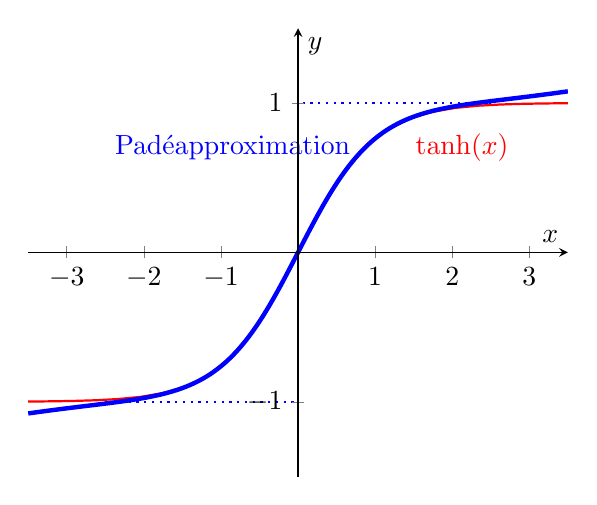
\begin{tikzpicture}
	\begin{axis}[
		xmin=-3.5, xmax=3.5,
		ymin=-1.5, ymax=1.5,
		axis lines=center,
		axis on top=true,
		domain=-3.5:3.5,
		ylabel=$y$,
		xlabel=$x$,
		]
		
		\addplot [mark=none,draw=red,thick] {tanh(\x)};
		\node [right, red] at (axis cs: 1.4,0.7) {$\tanh(x)$};
		\addplot [mark=none,draw=blue,ultra thick, samples=100, smooth] expression{x*(15+x^2)/(15+6*x^2)};
		\node [right, blue] at (axis cs: -2.5,0.7) {Padéapproximation};
		
		%% Add the asymptotes
		\draw [blue, dotted, thick] (axis cs:-2.5,-1)-- (axis cs:0,-1);
		\draw [blue, dotted, thick] (axis cs:+2.5,+1)-- (axis cs:0,+1);
	\end{axis}
\end{tikzpicture}
\caption{$[3 / 2]_{tanh}(x)$
\label{motivation:figure:Pade32}}
\end{figure}

\subsection{Vor- und Nachteile}
Der Fehler der Padé-Approximation wächst im Gegensatz zur
Taylor-Approximation zwar immer noch an, aber wesentlich weniger
schnell.
Im Beispiel wächst der Wert der Padé-Approximation linear mit $x$.
Dadurch ist die Approximation für einen wesentlich grösseren Bereich 
von Argumenten $x$ brauchbar.
Solange die Argumente in diesem Bereich bleiben, wird 
approximierende Funktion immer noch zu vergleichbaren Resultaten
führen.
Der Rechenaufwand ist dabei immer noch vergleichbar mit dem
der Taylor-Approximation.

